\documentclass[11pt]{article}
\usepackage[textwidth=18.0cm, textheight=23.0cm, top=2.0cm]{geometry}
\usepackage{pst-all}
\usepackage{amssymb}
\usepackage{tikz}
\usepackage{underscore}\begin{document}
\pagestyle{empty}


ClassName: \underline{\textbf{Class_05.2bp-1}}
\par
BinSize: \underline{\textbf{100 × 100}}
\par
ReduceSize: \underline{\textbf{100 × 100}}
\par
TypeNum: \underline{\textbf{20}}
\par
Num: \underline{\textbf{20}}
\par
OutS: \underline{\textbf{50000}}
\par
InS: \underline{\textbf{32367}}
\par
Rate: \underline{\textbf{0.647}}
\par
UB: \underline{\textbf{5}}
\par
LB0: \underline{\textbf{5}}
\par
LB: \underline{\textbf{5}}
\par
LBWithCut: \underline{\textbf{5}}
\par
NodeCut: \underline{\textbf{0}}
\par
ExtendedNodeCnt: \underline{\textbf{1}}
\par
GenNodeCnt: \underline{\textbf{1}}
\par
PrimalNode: \underline{\textbf{0}}
\par
ColumnCount: \underline{\textbf{5}}
\par
TotalCutCount: \underline{\textbf{0}}
\par
RootCutCount: \underline{\textbf{0}}
\par
LPSolverCnt: \underline{\textbf{1}}
\par
PricingSolverCnt: \underline{\textbf{0}}
\par
BranchAndBoundNum: \underline{\textbf{1}}
\par
isOpt: \underline{\textbf{true}}
\par
TimeOnPrimal: \underline{\textbf{0.000 s}}
\par
TimeOnPricing: \underline{\textbf{0.000 s}}
\par
TimeOnRmp: \underline{\textbf{0.079 s}}
\par
TotalTime: \underline{\textbf{0.141 s}}
\par
\newpage


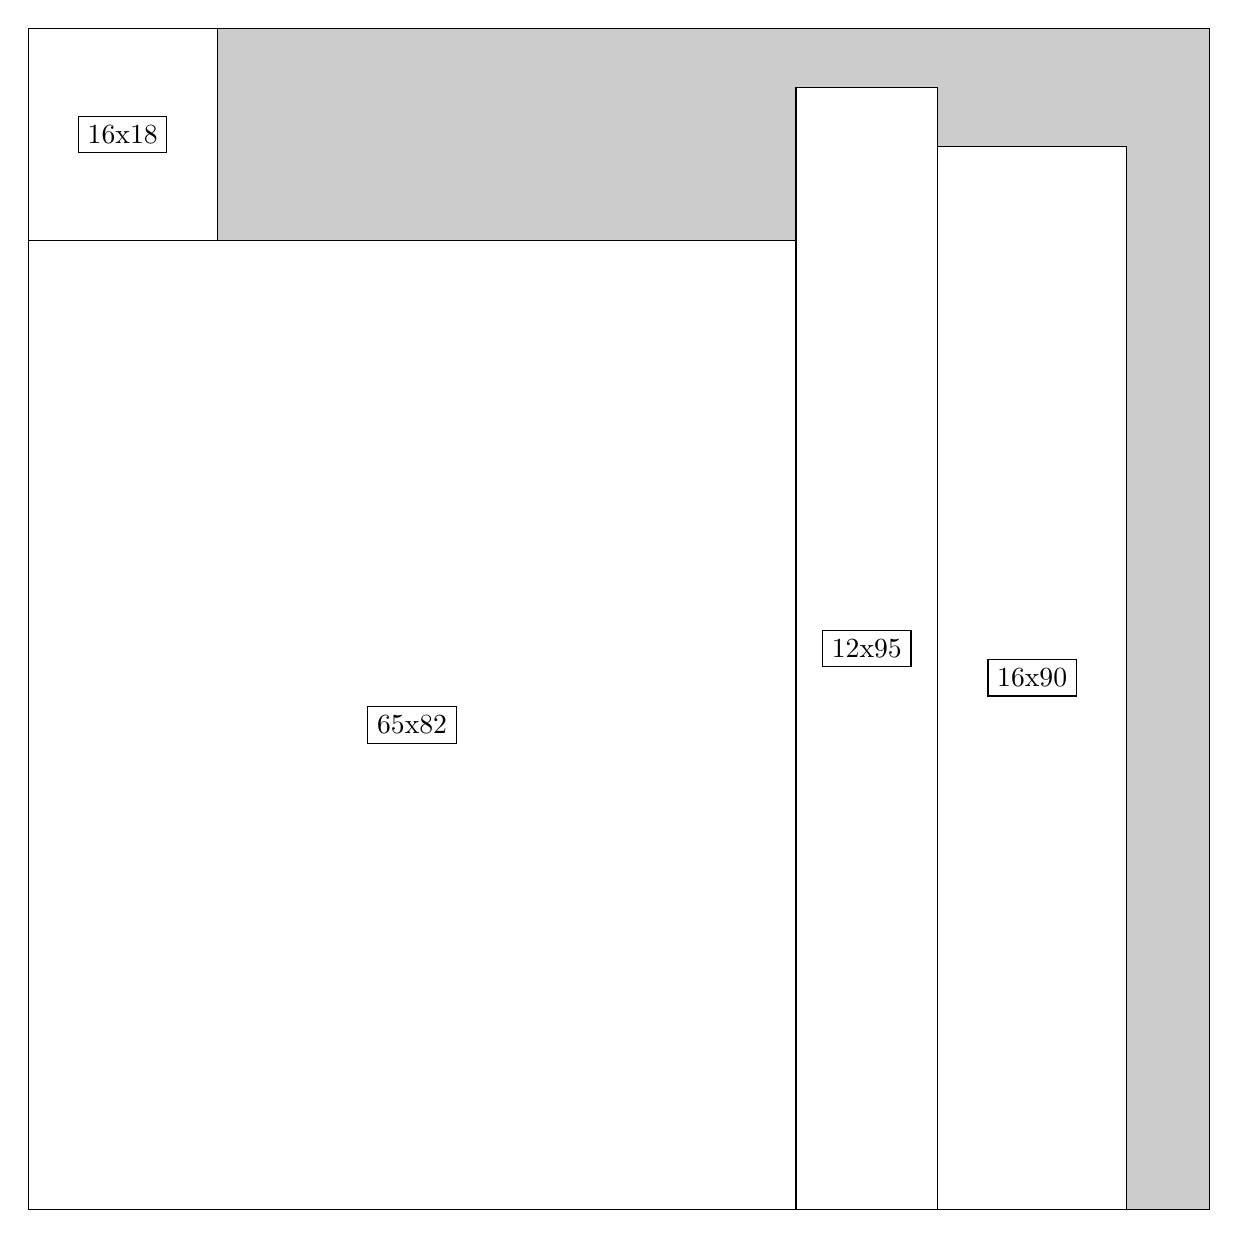
\begin{tikzpicture}[shorten >=1pt,scale=1.0,every node/.style={scale=1.0},->]
\tikzstyle{vertex}=[circle,fill=black!25,minimum size=14pt,inner sep=0pt]
\filldraw[fill=gray!40!white, draw=black] (0,0) rectangle (15.0,15.0);
\foreach \name/\x/\y/\w/\h in {12x95/9.75/0.0/1.7999999999999998/14.25,65x82/0.0/0.0/9.75/12.299999999999999,16x90/11.549999999999999/0.0/2.4/13.5,16x18/0.0/12.299999999999999/2.4/2.6999999999999997}
\filldraw[fill=white!40!white, draw=black] (\x,\y) rectangle node[draw] (\name) {\name} ++(\w,\h);
\end{tikzpicture}


w =12 , h =95 , x =65 , y =0 , v =1140
\par
w =65 , h =82 , x =0 , y =0 , v =5330
\par
w =16 , h =90 , x =77 , y =0 , v =1440
\par
w =16 , h =18 , x =0 , y =82 , v =288
\par
\newpage


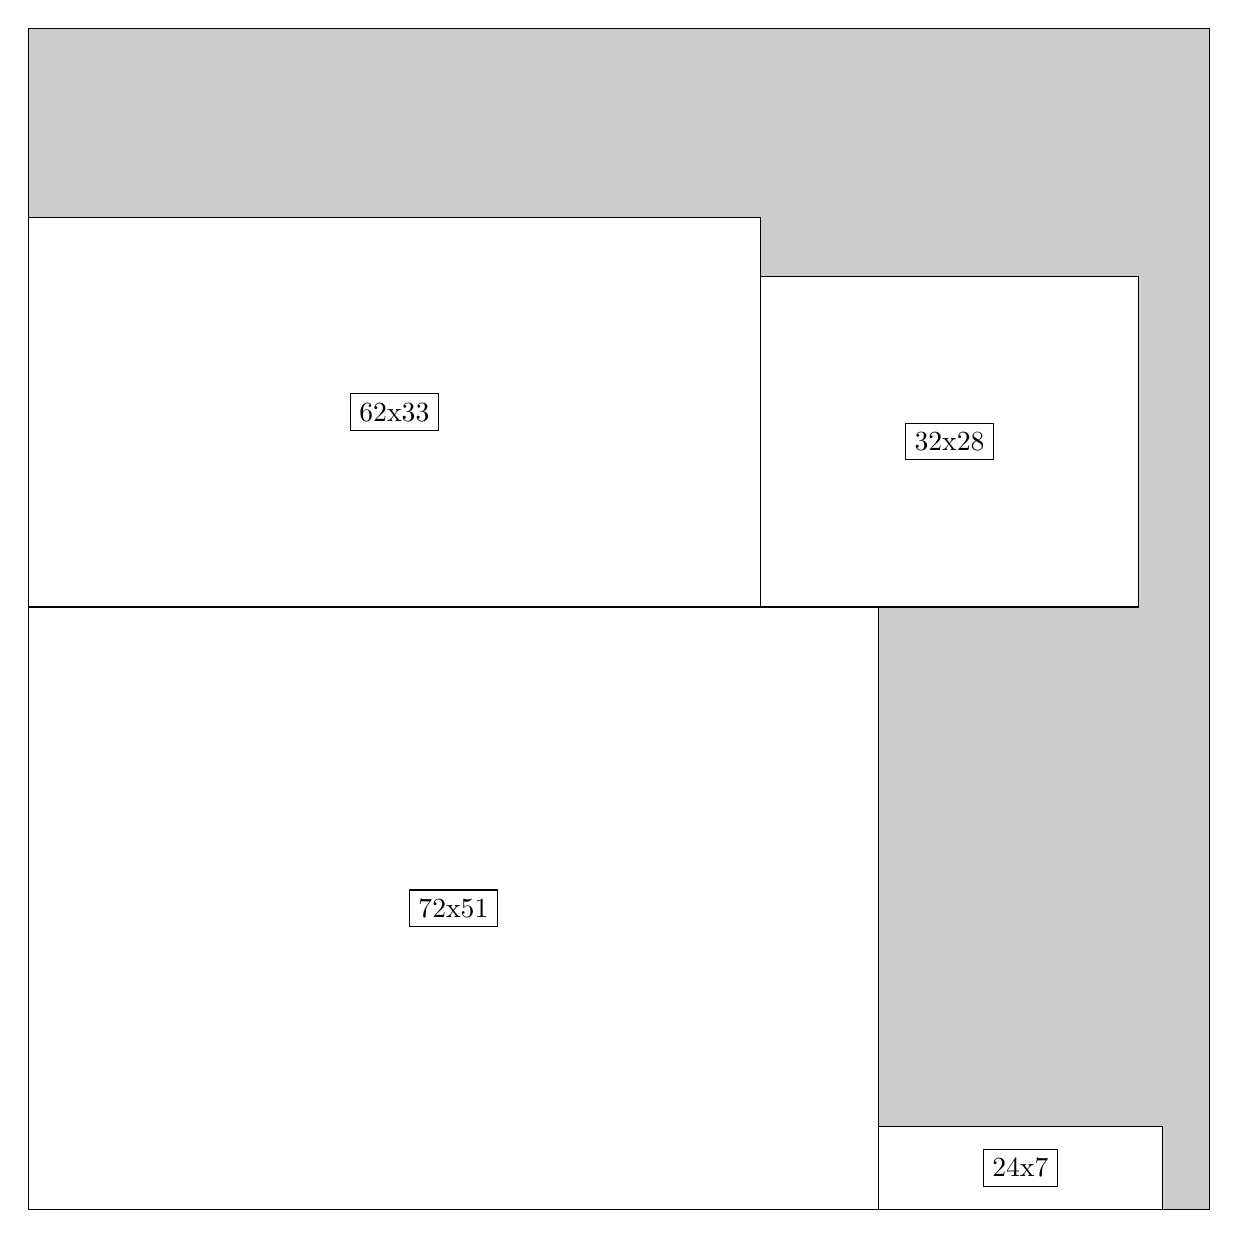
\begin{tikzpicture}[shorten >=1pt,scale=1.0,every node/.style={scale=1.0},->]
\tikzstyle{vertex}=[circle,fill=black!25,minimum size=14pt,inner sep=0pt]
\filldraw[fill=gray!40!white, draw=black] (0,0) rectangle (15.0,15.0);
\foreach \name/\x/\y/\w/\h in {72x51/0.0/0.0/10.799999999999999/7.6499999999999995,62x33/0.0/7.6499999999999995/9.299999999999999/4.95,32x28/9.299999999999999/7.6499999999999995/4.8/4.2,24x7/10.799999999999999/0.0/3.5999999999999996/1.05}
\filldraw[fill=white!40!white, draw=black] (\x,\y) rectangle node[draw] (\name) {\name} ++(\w,\h);
\end{tikzpicture}


w =72 , h =51 , x =0 , y =0 , v =3672
\par
w =62 , h =33 , x =0 , y =51 , v =2046
\par
w =32 , h =28 , x =62 , y =51 , v =896
\par
w =24 , h =7 , x =72 , y =0 , v =168
\par
\newpage


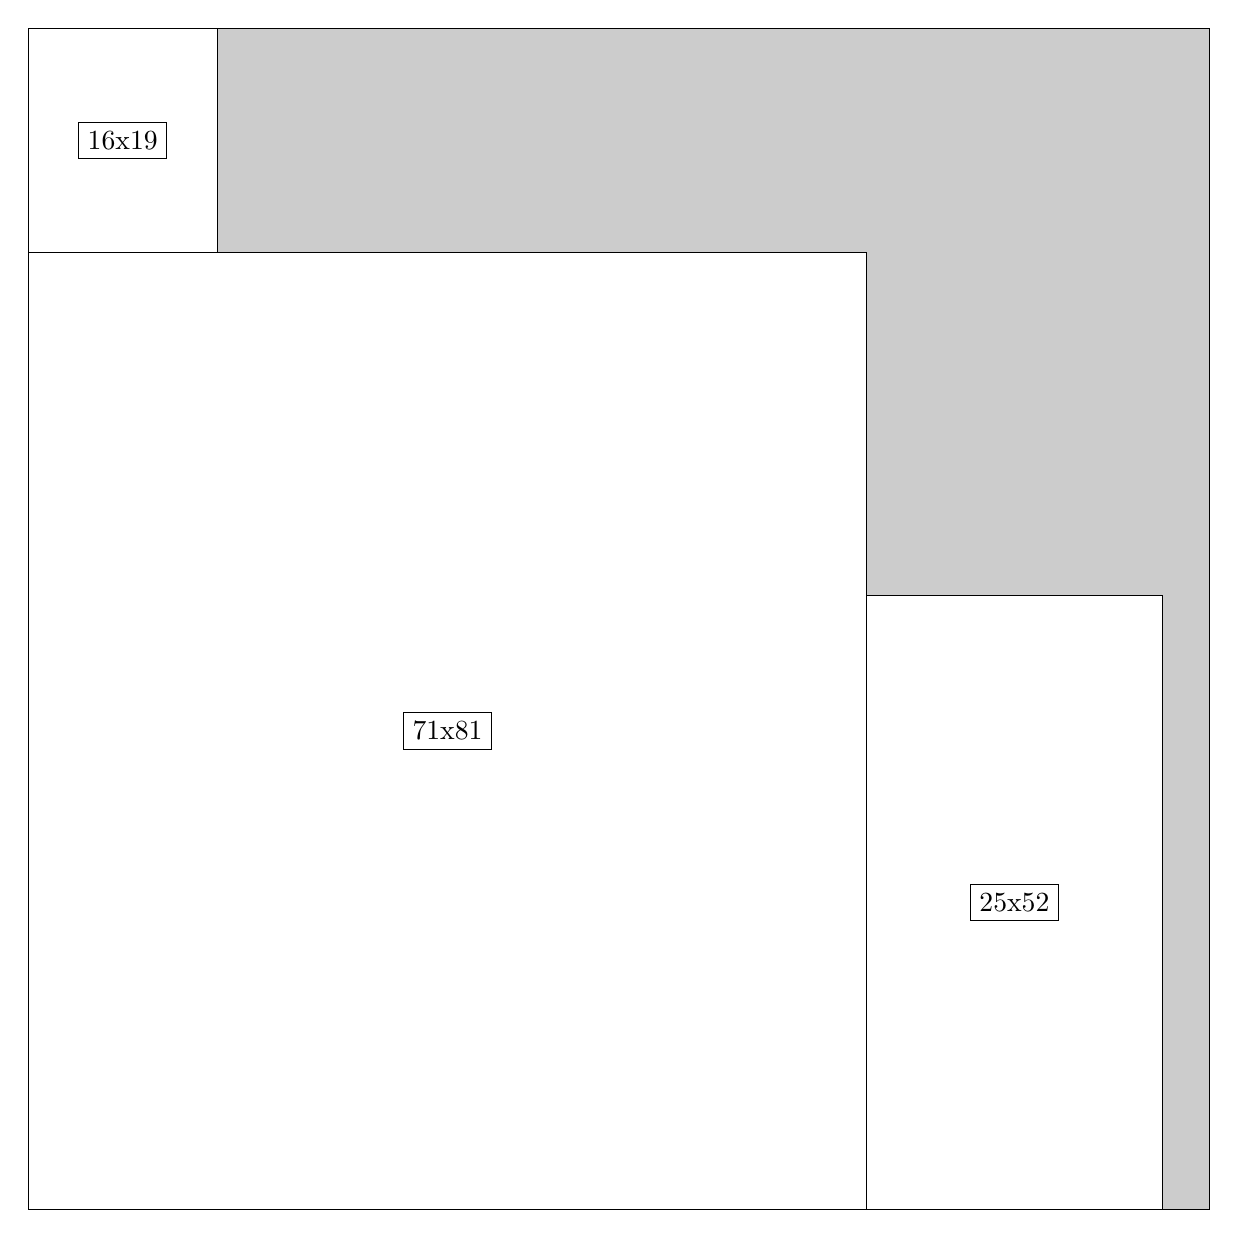
\begin{tikzpicture}[shorten >=1pt,scale=1.0,every node/.style={scale=1.0},->]
\tikzstyle{vertex}=[circle,fill=black!25,minimum size=14pt,inner sep=0pt]
\filldraw[fill=gray!40!white, draw=black] (0,0) rectangle (15.0,15.0);
\foreach \name/\x/\y/\w/\h in {25x52/10.65/0.0/3.75/7.8,71x81/0.0/0.0/10.65/12.15,16x19/0.0/12.15/2.4/2.85}
\filldraw[fill=white!40!white, draw=black] (\x,\y) rectangle node[draw] (\name) {\name} ++(\w,\h);
\end{tikzpicture}


w =25 , h =52 , x =71 , y =0 , v =1300
\par
w =71 , h =81 , x =0 , y =0 , v =5751
\par
w =16 , h =19 , x =0 , y =81 , v =304
\par
\newpage


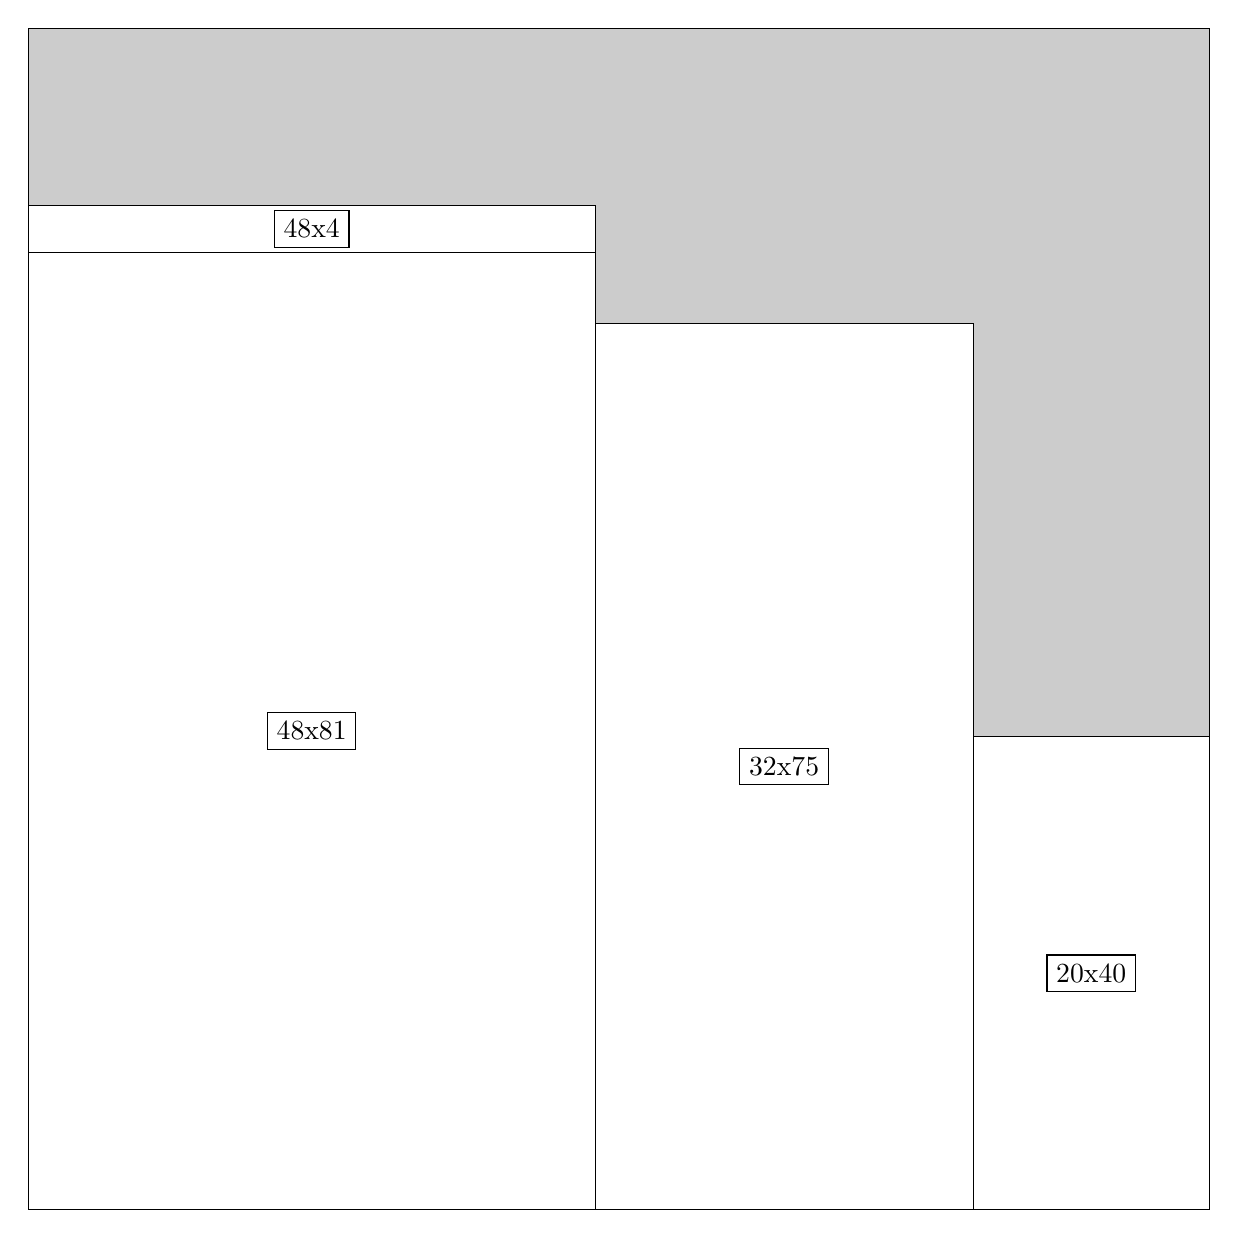
\begin{tikzpicture}[shorten >=1pt,scale=1.0,every node/.style={scale=1.0},->]
\tikzstyle{vertex}=[circle,fill=black!25,minimum size=14pt,inner sep=0pt]
\filldraw[fill=gray!40!white, draw=black] (0,0) rectangle (15.0,15.0);
\foreach \name/\x/\y/\w/\h in {48x81/0.0/0.0/7.199999999999999/12.15,32x75/7.199999999999999/0.0/4.8/11.25,20x40/12.0/0.0/3.0/6.0,48x4/0.0/12.15/7.199999999999999/0.6}
\filldraw[fill=white!40!white, draw=black] (\x,\y) rectangle node[draw] (\name) {\name} ++(\w,\h);
\end{tikzpicture}


w =48 , h =81 , x =0 , y =0 , v =3888
\par
w =32 , h =75 , x =48 , y =0 , v =2400
\par
w =20 , h =40 , x =80 , y =0 , v =800
\par
w =48 , h =4 , x =0 , y =81 , v =192
\par
\newpage


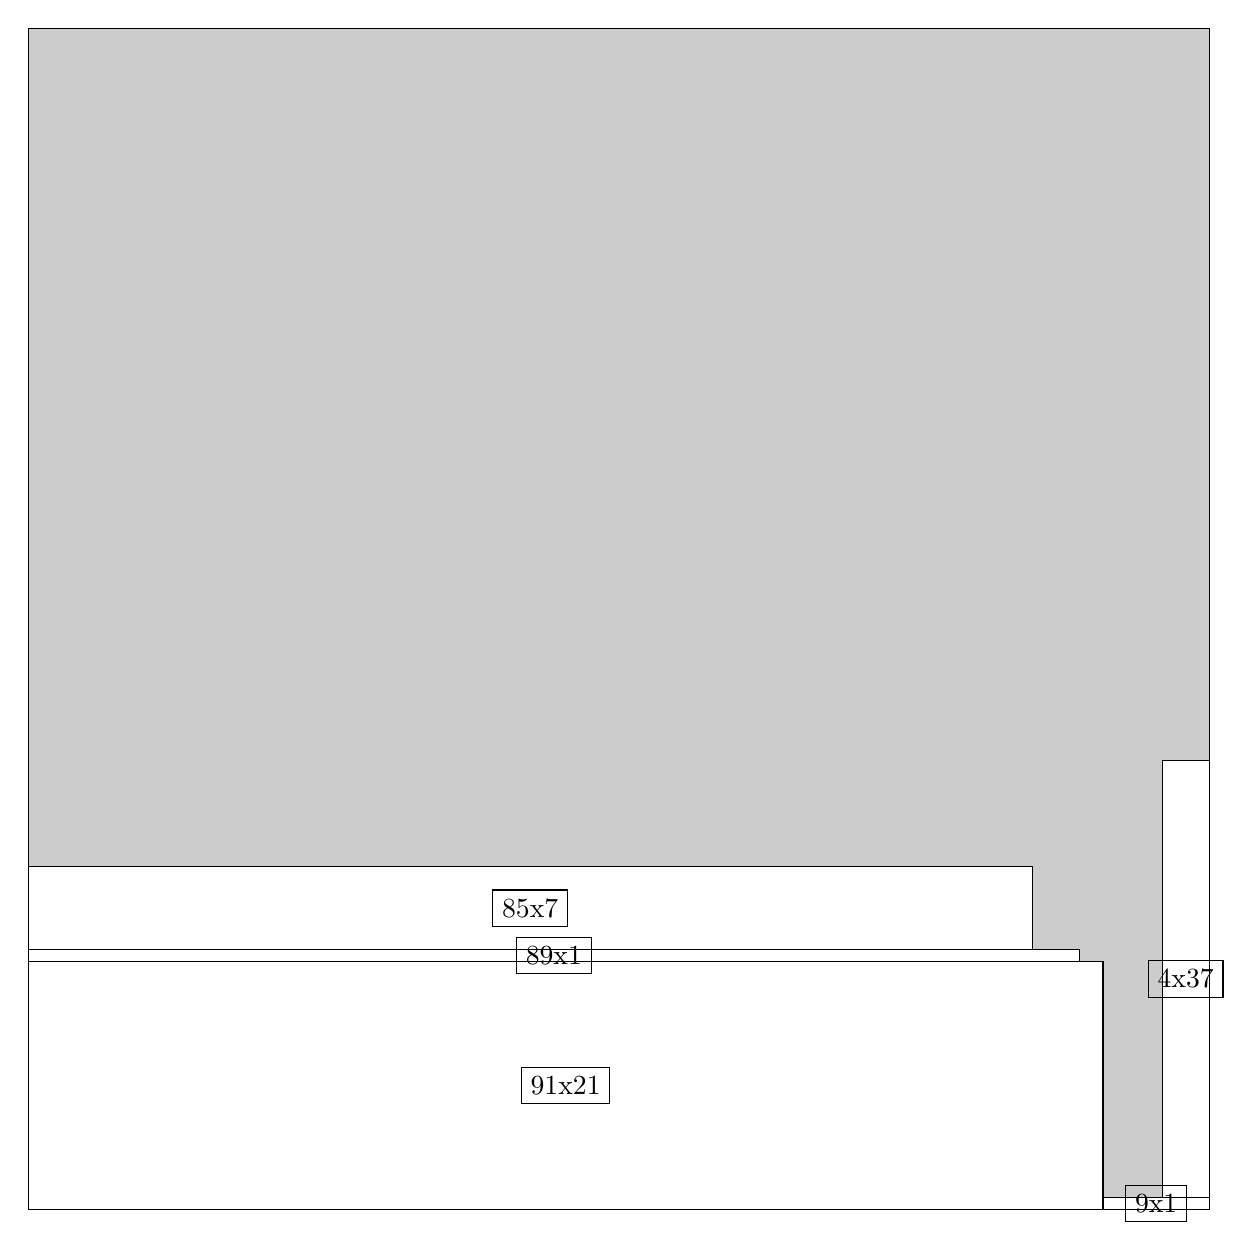
\begin{tikzpicture}[shorten >=1pt,scale=1.0,every node/.style={scale=1.0},->]
\tikzstyle{vertex}=[circle,fill=black!25,minimum size=14pt,inner sep=0pt]
\filldraw[fill=gray!40!white, draw=black] (0,0) rectangle (15.0,15.0);
\foreach \name/\x/\y/\w/\h in {91x21/0.0/0.0/13.65/3.15,85x7/0.0/3.3/12.75/1.05,4x37/14.399999999999999/0.15/0.6/5.55,89x1/0.0/3.15/13.35/0.15,9x1/13.65/0.0/1.3499999999999999/0.15}
\filldraw[fill=white!40!white, draw=black] (\x,\y) rectangle node[draw] (\name) {\name} ++(\w,\h);
\end{tikzpicture}


w =91 , h =21 , x =0 , y =0 , v =1911
\par
w =85 , h =7 , x =0 , y =22 , v =595
\par
w =4 , h =37 , x =96 , y =1 , v =148
\par
w =89 , h =1 , x =0 , y =21 , v =89
\par
w =9 , h =1 , x =91 , y =0 , v =9
\par
\newpage


\end{document}